\chapter{Strumenti e tecnologie}
\label{cha:intro}
\vspace{5mm}

\emph{Questo capitolo descrive in maniera più approfondita le tecnologie utilizzate nella prima e nella seconda versione in un confronto dettagliato.}

\section{Tecnologie utilizzate in Open Air Museum}\vspace{5mm}

Indicherò le varie tecnologie utilizzate per l'attuale versione dell'applicativo.\vspace{5mm}

\subsection{Filemaker}\vspace{5mm}

Filemaker è una piattaforma per creare applicativi personalizzati votati alla categoria “gestionale” sviluppata da Apple. Open Air Museum utilizza questa tecnologia per creare l’interfaccia per la raccolta dati che verrà utilizzata da alcuni addetti comunali che appunto arricchiranno l’applicativo con i testi e i media provenienti da questo software. Tale applicativo è standalone e quindi slegato dall’applicativo lato server che espone le Api e l’importazione dei dati provenienti da questa soluzione deve essere fatta manualmente. Ciò comporta uno svantaggio non indifferente che preclude una scalabilità rapida del prodotto. La scelta di questa tecnologia era quella di avere il più rapidamente possibile un prodotto in grado di iniziare a raccogliere dati il prima possibile e qualunque altra soluzione, seppur migliore in un ottica futura, avrebbe impiegato maggior tempo di sviluppo.\vspace{5mm}

\subsection{Node Js}\vspace{5mm}

	Come descritto in precedenza, Node js è un runtime di Javascript al di fuori del browser.Tale programma, come dicuterò più avanti, utilizza Chrome V8\cite{V8} come motore per eseguire Javascript ed grazie ciò NodeJs è stato fornito di una suite di interfacce per la comunicazione con l'hardware. In particolare questa particolare implementazione viene indicata come I/O non bloccante\cite{AsincIO}. La particolarità di questa soluzione è che mette a disposizione una serie di Api a basso livello che permettono di utilizzare la scheda di rete e quindi di avviare server TCP e HTTP oltre che accesso al file system quindi lettura e scrittura su disco. In Open air museum questo framework è utilizzato per costruire il lato server ed esporre una serie di Api Http Rest che permettono la fruizione dei dati. Tutti i media, quindi audio e immagini vengono serviti anch’essi da questa piattaforma che oltre a questo gestisce anche l’autenticazione degli utenti e la gestione degli stessi. \vspace{5mm}
	
	\subsection{Estimote}\vspace{5mm}
	
	\subsection{Developer Tools}\vspace{5mm}
	
	[RISCRIVI QUESTA PARTE.]

	Xcode è una Ide per lo sviluppo IOS. L’applicativo per tale sistema operativo è stato sviluppato in Swift4.\vspace{5mm}

	Android Studio è una Ide per lo sviluppo Android. L’applicativo per tale sistema operativo è stato sviluppato in Java per android.\vspace{5mm}

	MySql/SqLite sono le tecnologie che utilizzano i due database relazionali di cui il prodotto è fornito. Tutti i dati lato server sono contenuti in un database MySql che viene pilotato tramite l’applicativo lato server in Nodejs. Entrambi i database lato client utilizzano invece SqLite. 
	
	Visual Studio Code
	
	Github
	
	Bitbucket?
	
		\subsection{Modello ER}\vspace{5mm}
		
	Lo schema relazionale per il lato server è il seguente, si vedano gli allegati per i due(???) schemi ER corrispondenti. [ESPANDI?]  \vspace{5mm}
	
\begin{figure}[h]
\centering
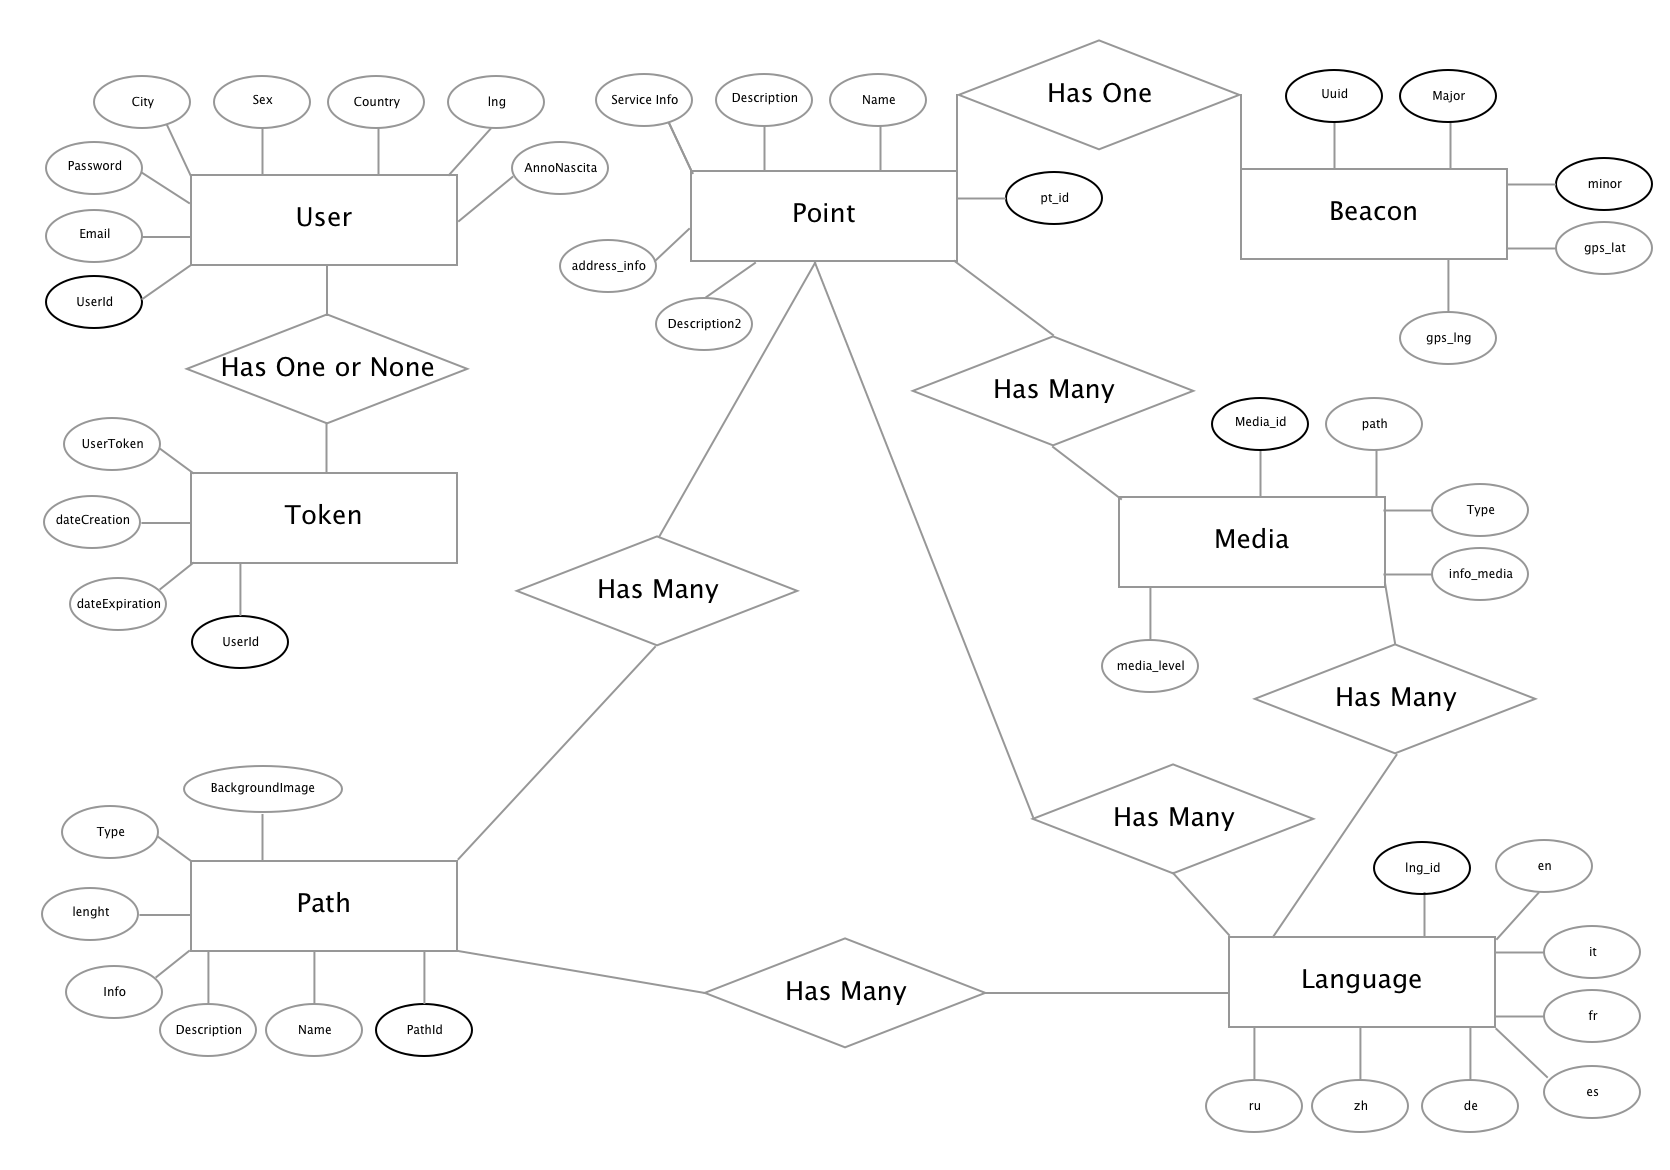
\includegraphics[width=0.9\textwidth]{images/erOld.png}
\caption{Schema ER vecchia versione}
\end{figure}
\vspace{5mm}

[mi sa che manca uno schema.]
	
\section{Tecnologie versione 2.0}\vspace{5mm}
Indicherò le varie tecnologie utilizzate per la nuova versione dell'applicativo ponendo particolare attenzione a che vantaggi portano.\vspace{5mm}

	\subsection{React}\vspace{5mm}

React è una Libreria Javascript per lo sviluppo di interfacce grafiche a componenti, permette lo sviluppo di single page application (SPA). In Alakai l’applicativo che permette l’inserimento dei dati e dei media oltre alle descrizioni dei punti di interesse e dei percorsi è creata utilizzando questa tecnologia sfruttando un set di Api che il lato server fornisce. Questo centralizza la gestione dei dati in un unico luogo e cioè il server, tale approccio permette di utilizzare l'applicativo backend come unica fonte di verità senza dover gestire due prodotti separati come vi era in precedenza. [ESPANDI!!!]\vspace{5mm}

	\subsection{Redux}\vspace{5mm}
	
	Redux è una libreria Javascript che permette di gestire lo stato applicativo come un unico oggetto statico, modificabile soltanto attraverso della azioni ben definite applicate ad esso. Ogni modifica viene fatta attraverso una funzione pura\cite{PureFunction} chiamata reducer che modifica a seconda dell'implementazione una parte specifica dello store. La firma di tale funzione prende due parametri, il primo è l'oggetto che rappresenta lo stato attuale dell'applicativo, il secondo è ciò che rappresenta l'azione che si sta compiendo. Tale azione dovrà sempre possedere una tipologia mentre può o non può avere un payload di dati che si riferiscono a quell'azione specifica. Ciò che ritornerà il reducer sarà un oggetto che diventerà il nuovo stato applicativo. Questa tecnologia è utilizzata per gestire i dati che gli applicativi mobile recupereranno dal server in modo predittivo e sicuro. Tale implementazione permette di evitare side effects\cite{SideEffects} nello stato applicativo facendo si che l'unica fonte di verità sia sempre affidabile e prevedibile.  [ESPANDI!!!] \vspace{5mm}
	
\begin{figure}[h]
\centering
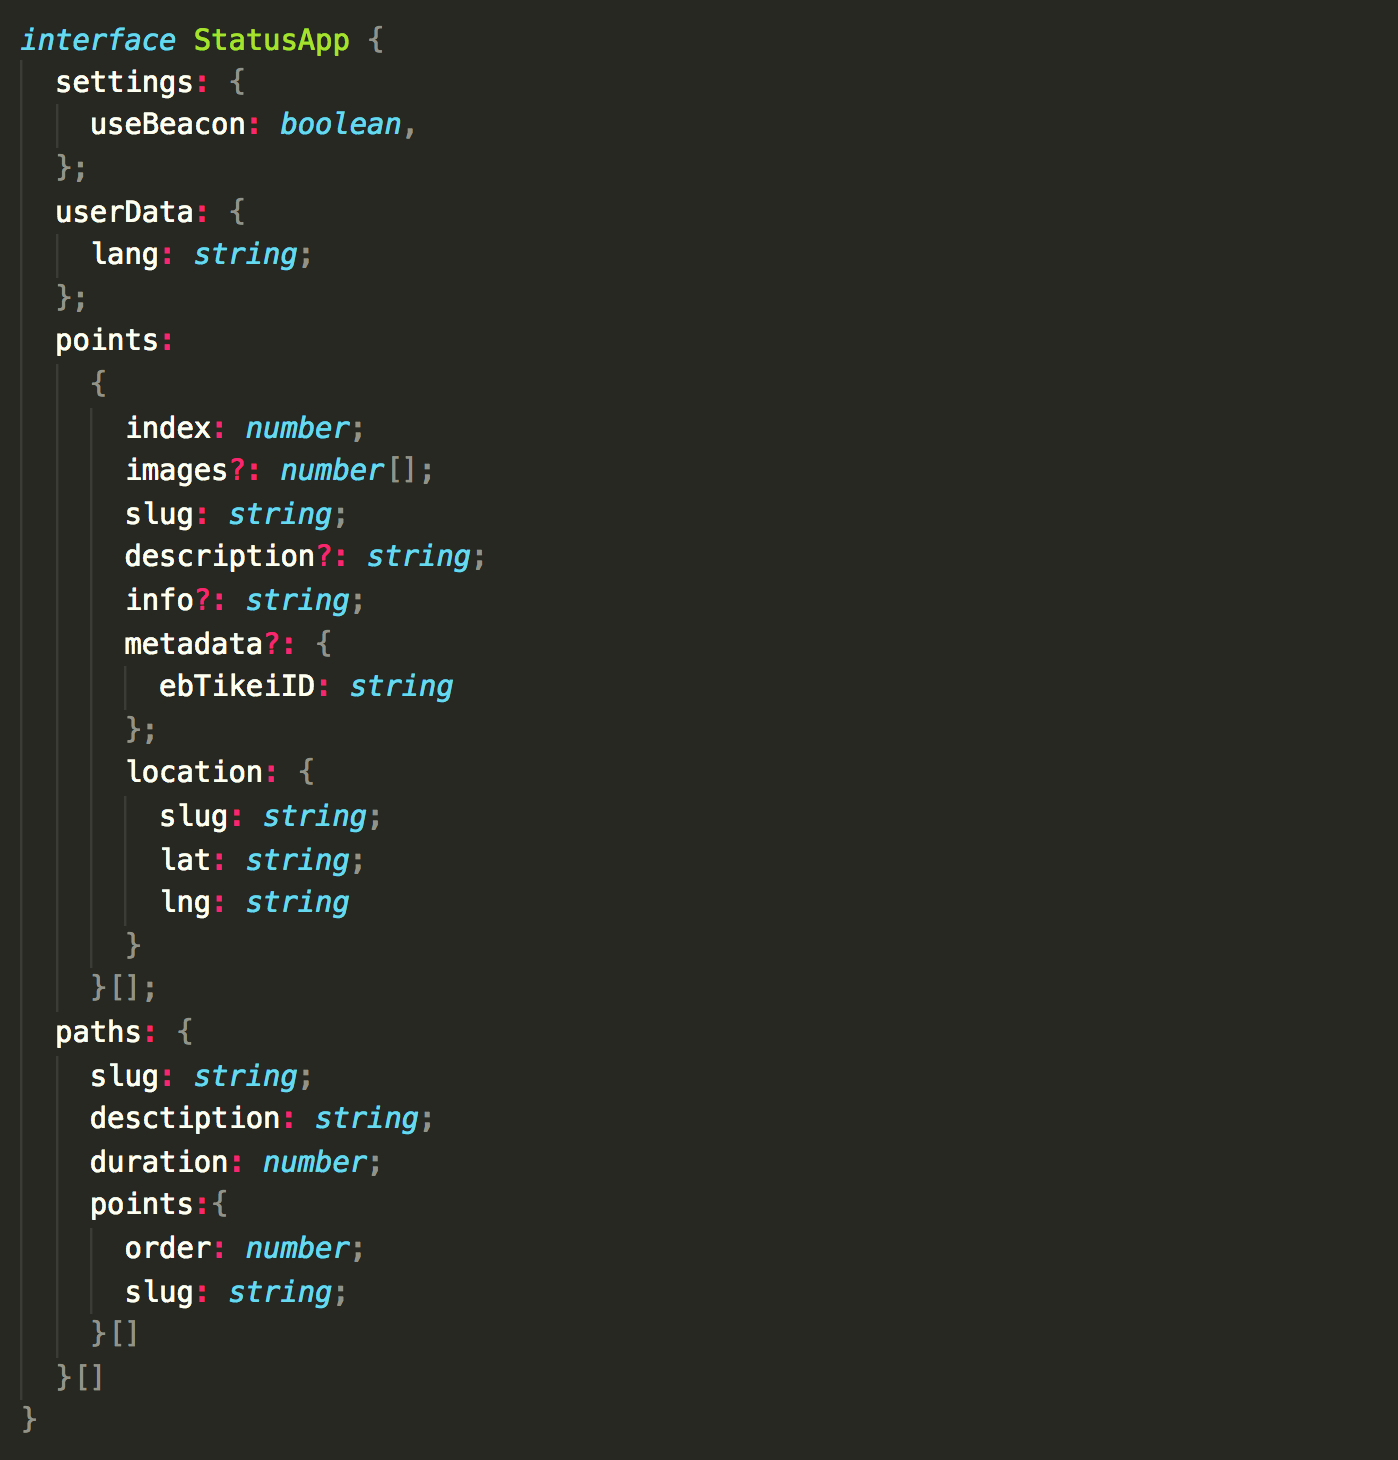
\includegraphics[width=0.7\textwidth]{images/store.png}
\caption{Interfaccia Store Redux}
\end{figure}
\vspace{5mm}

\subsection{React-Native}\vspace{5mm}

	React-Native è l'implementazione di React ma per l’ambiente nativo. Questa tecnologia verrà usata per creare l’interfaccia e la logica degli applicativi IOS e Android. Tale scelta infatti permette di condividere buona parte del codice tra le due piattaforme.\vspace{5mm}

\subsection{Express}\vspace{5mm}

	Express è l'implementazione del pattern middleware per Node Js. Tale framework permette di gestire con granularità il routing delle Api e da la possibilità di centralizzare la gestione degli errori. L'implementazione di tale pattern si riflette in un applicativo che esegue le computazioni attraverso una cascata di funzioni chiamate una dopo l'altra in ordine, ed ognuna di esse ha la facoltà di decidere se continuare la catena o interrompere la computazione. Questo permette di avere una struttura affidabile per gestire il routeing delle Rest api rendendo molto veloce e predittivo lo sviluppo.\vspace{5mm}

\subsection{SqLite}\vspace{5mm}

	SqLite è “File-based” database utilizzato lato server per il salvataggio delle informazioni fornite dagli utenti admin attraverso l’applicativo web per la raccolta dei dati. Tale scelta è stata fatta per la flessibilità di questa tecnologia che permette di gestire internamente all’applicativo la creazione dello stesso e non attraverso una dipendenza esterna. Questo è stato fatto per semplificare ulteriormente il deploy eliminando le necessità di aggiungere una configurazione ulteriore all’ambiente.\vspace{5mm}
	
	\subsection{Modello ER}\vspace{5mm}

Ora descriverò brevemente il nuovo schema logico dell'applicativo e come le varie tecnologie, tutte basate su Javascript interagiscono fra loro.
	
\begin{figure}[h]
\centering
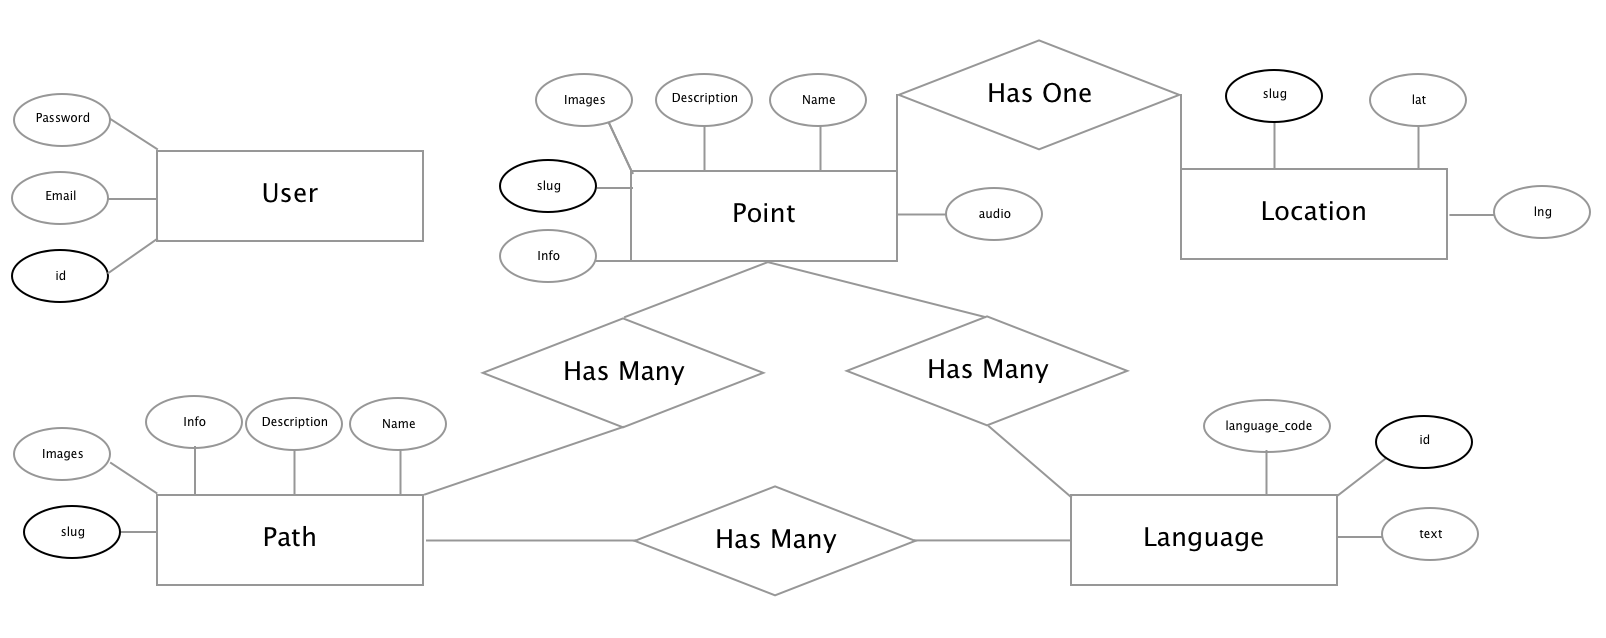
\includegraphics[width=0.9\textwidth]{images/erNew.png}
\caption{Schema ER nuova versione}
\end{figure}
	
	
\begin{figure}[h]
\centering
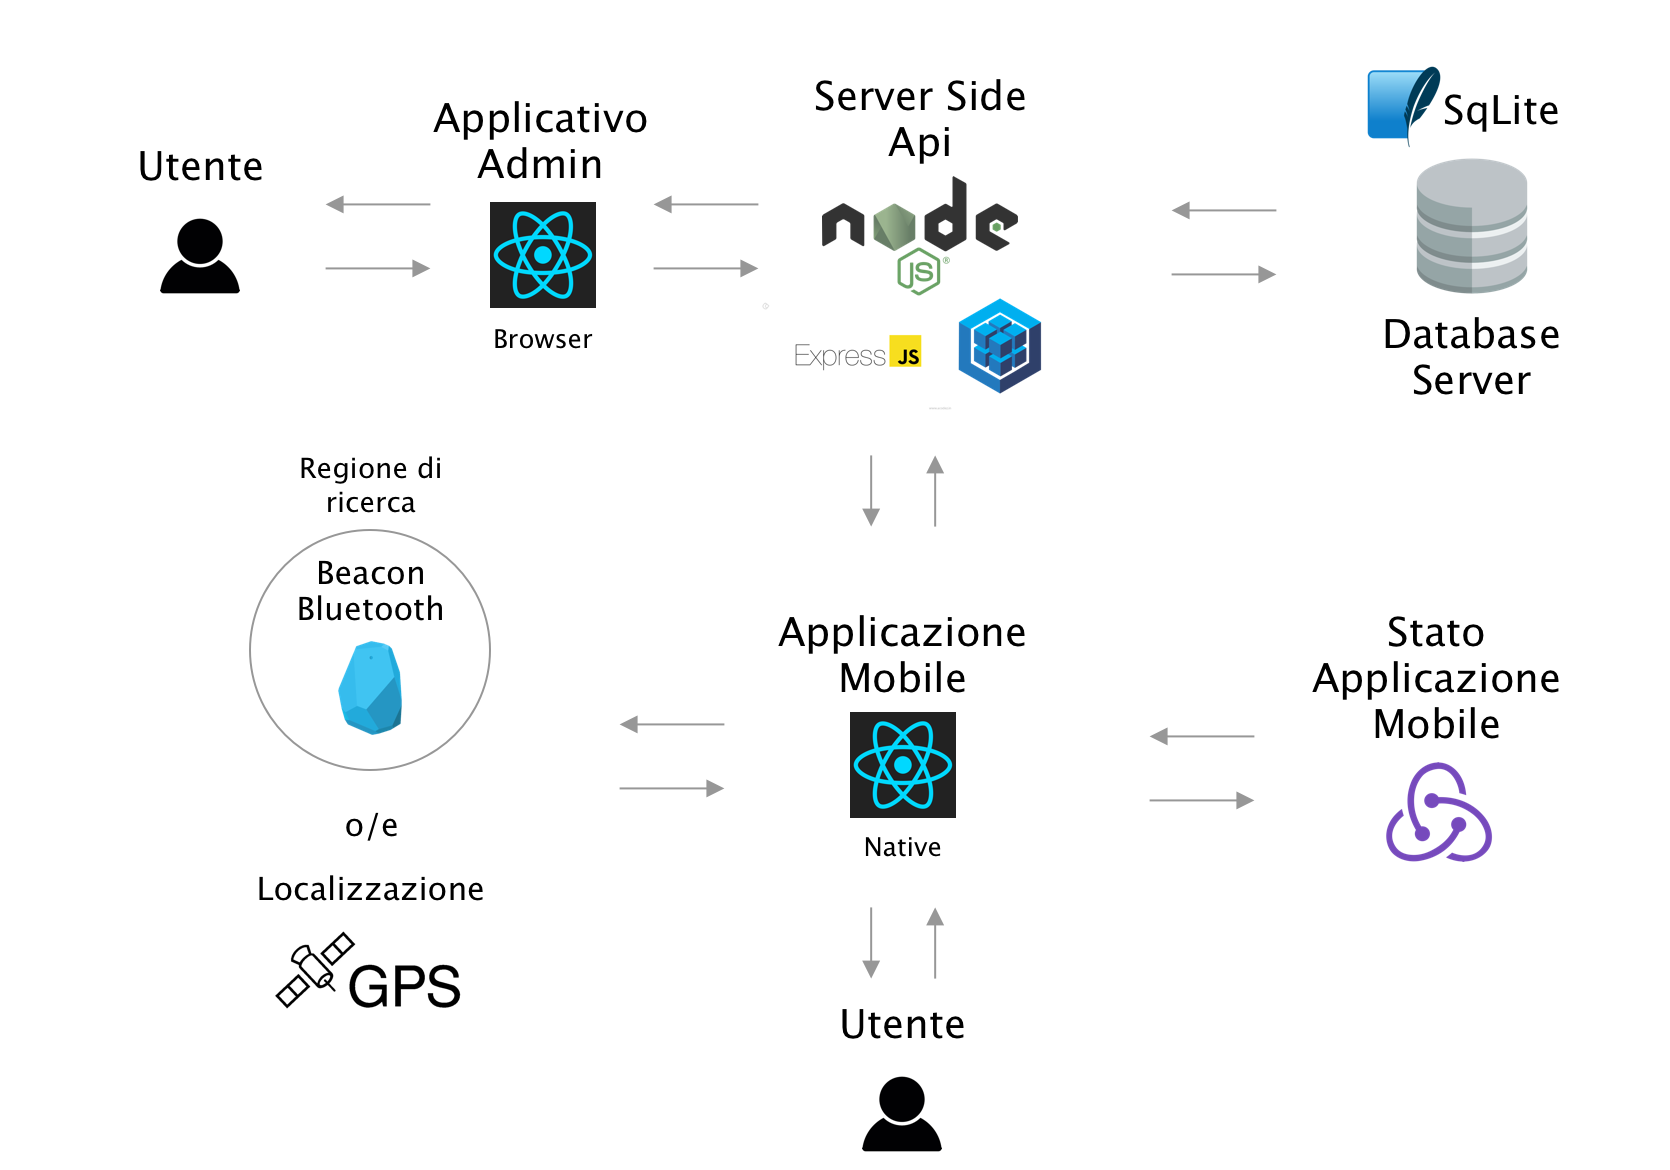
\includegraphics[width=0.9\textwidth]{images/stackAlakai.png}
\caption{Schema stack nuova versione}
\end{figure}

\vspace{5mm}Come si può vedere in figura 2.4 lo stack risulta meno complesso e vanta l'utilizzo di meno tecnologie per raggiungere le medesime funzionalità. Come si può notare i punti di interazione con la piattaforma sono gestiti da due applicativi basati entrambi su React, il primo è l'applicativo mobile che utilizza React-native mentre il secondo è la webApp admin. Entrambi questi applicativi ricevono input dall'utente ma il primo utilizza hardware esterno per arricchire la propria raccolta informazioni con la posizione dell'utente, ricevuta attraverso il gps o Beacon bluethoot. Tali applicativi interagiscono con il server mediante delle Rest Api che, come nella versione precedente, forniscono i dati sui punti e i percorsi; ma, in contrasto con l'applicativo prima del refactor, portano anche la configurazione impostata dall'applicativo admin in modo da adattarlo alle richieste di chi gestisce i punti e i percorsi. Tali dati vengono salvati in un database SqLite il cui unico punto di accesso è attraverso le api fornite dal server. \vspace{5mm}

Tale approccio garantisce che i dati siano sempre consistenti con quello che è l'applicativo server in modo da mantenere la struttura consistente con il versionamento del prodotto. Un ulteriore struttura per mantenere i dati è presente a lato mobile mediante Redux, questo è utile per poter salvare le configurazioni e mantenerle tali in modo consistente attraverso l'app in modo da creare una coesione tra tutti i componenti di React che necessitano di usufruire dei dati. Tale stato applicativo viene idratato attraverso le api Rest e quando questo non è possibile per mancanza di rete permette di utilizzare tramite React-native lo Storage locale del dispositivo come luogo di backup. Ogni mutazione dello stato applicativo viene infatti seguita da un operazione asincrona che ha lo scopo di salvare uno snapshot dello store nella memoria del dispositivo in modo da poter essere sempre consistente nel mostrare gli ultimi dati disponibili anche se il dispositivo risulta offline.\vspace{5mm}

\section{Confronto tra le due versioni}\vspace{5mm}  
[forse questo va piu nelle conclusioni?]

Confrontando gli stack delle due applicazioni in termini di tecnologie utilizzate possiamo vedere i motivi per cui le scelte fatte migliorano il software e sotto quali aspetti. \vspace{5mm}

Grazie all'utilizzo del medesimo framework lato mobile e lato web è stato possibile condividere gran parte del codice e delle logiche di interazione con le api lato server. Un altra zona di condivisione è l'implementazione di Redux. Data la sua agnosticità sulla piattaforma utilizzata questa libreria è un perfetto esempio di come l'utilizzo di uno stack basato interamente su Javascript porti ad un riutilizzo del codice in modo importante ma sopratutto in modi impraticabili precedentemente. In particolare tra l’applicativo admin sviluppato come webapp per il browser e gli applicativi nativi ho condiviso la totalità dell’implementazione gestendo lo store allo stesso modo. Le differenze principali sono sulla libreria che permette di interfacciarsi con le api lato server. Seppur molti metodi sono condivisi, quelli relativi alla mutazione dei dati sono riserveti ai soli utenti autenticati e cioè Admin. Tale peculiarità però non influisce nella possibilità di riutilizzare parte della libreria che implementa sia i metodi lato amministratore che quelli lato utente senza privilegi.\vspace{5mm} 

Un ulteriore punto è che rispetto alla versione precedente vi è una somiglianza molto forte tra quello che è l’applicativo web e l’applicativo nativo, le due applicazioni non sono compatibili ma condividono gran parte delle logiche e dei pattern essendo di fatto lo stesso framework. Ciò permette di avere un livello di complessità all'approccio a questo progetto più bassa della versione precedente. Questo porta a tempi più corti per l'apprendimento dei pattern e delle logiche e di conseguenza risulta in una miglior produttività.\vspace{5mm}
	
La scelta dell’utilizzo di un database a file con la possibilità di configurare e passare ad un database “classico” si è rivelata molto importante per la scalabilità dell’applicativo. SqLite risulta più comodo in fase di deploy di contro, non ha le prestazioni di un database “classico” e la possibilità di configurare rapidamente la tecnologia da utilizzare è un plus importante. Questo si ottiene grazie all’impiego di un ORM in grado di fornire questa features come Sequelize. Oltre a questo permette di implementare in modo veloce migrazioni e seeder restando sempre agnostico sulla tecnologia a database. La versione precedente conteneva una pesante assunzione sull’utilizzo di un database MySql e ciò abbassava sostanzialmente la flessibilità e il riutilizzo del prodotto.\vspace{5mm}

Un altra differenza rispetto alla precedente è l’esistenza dell’applicativo admin in react che dovrà essere servito dall’applicativo server. Per fare questo è necessario che tutte le richieste non inviate direttamente a /api, vengano tutte reindirizzare all’applicativo in modo che la SPA utilizzi il router interno a React per mostrare i contenuti corrispondenti all’url della richiesta.\vspace{5mm}

Riguardo al lato “admin”, cioè quello che va a sostituire Filemaker nella raccolta dati, è stato sviluppato con React. La scelta di sviluppare una SPA\cite{SPA} per questo compito è stata dettata da un bisogno di rendere questa operazione iterabile e ripetibile. Nel caso in cui il cliente volesse cambiare dei testi o correggere delle traduzioni può farlo in autonomia, senza dover passare da una figura che traduca le modifiche richieste aggiungendole a database manualmente. Questo processo inoltre astrae ulteriormente la struttura del database durante il processo di inserimento dei dati offrendo quindi flessibilità su modifiche future alla struttura. Un altro punto a favore della scelta di una SPA \vspace{5mm}

